
Bounties are frequently used in some projects while rarely used in others (see Section~\ref{prestudy}). The frequency of using bounties in a project may reflect the degree of experience that the project has with bounties and may have an impact on the issue-addressing process.
Therefore, in this RQ, we investigate how the issue-addressing likelihood changes across different projects with different bounty-usage frequencies. Furthermore, we study the relationship of the issue-addressing likelihood with the bounty value and the project activities (e.g., creating pull requests).
With a better understanding of the bounty across different projects, we can provide insights on how to better use bounties.% for a wide range of projects.



\begin{figure}[t]
\centering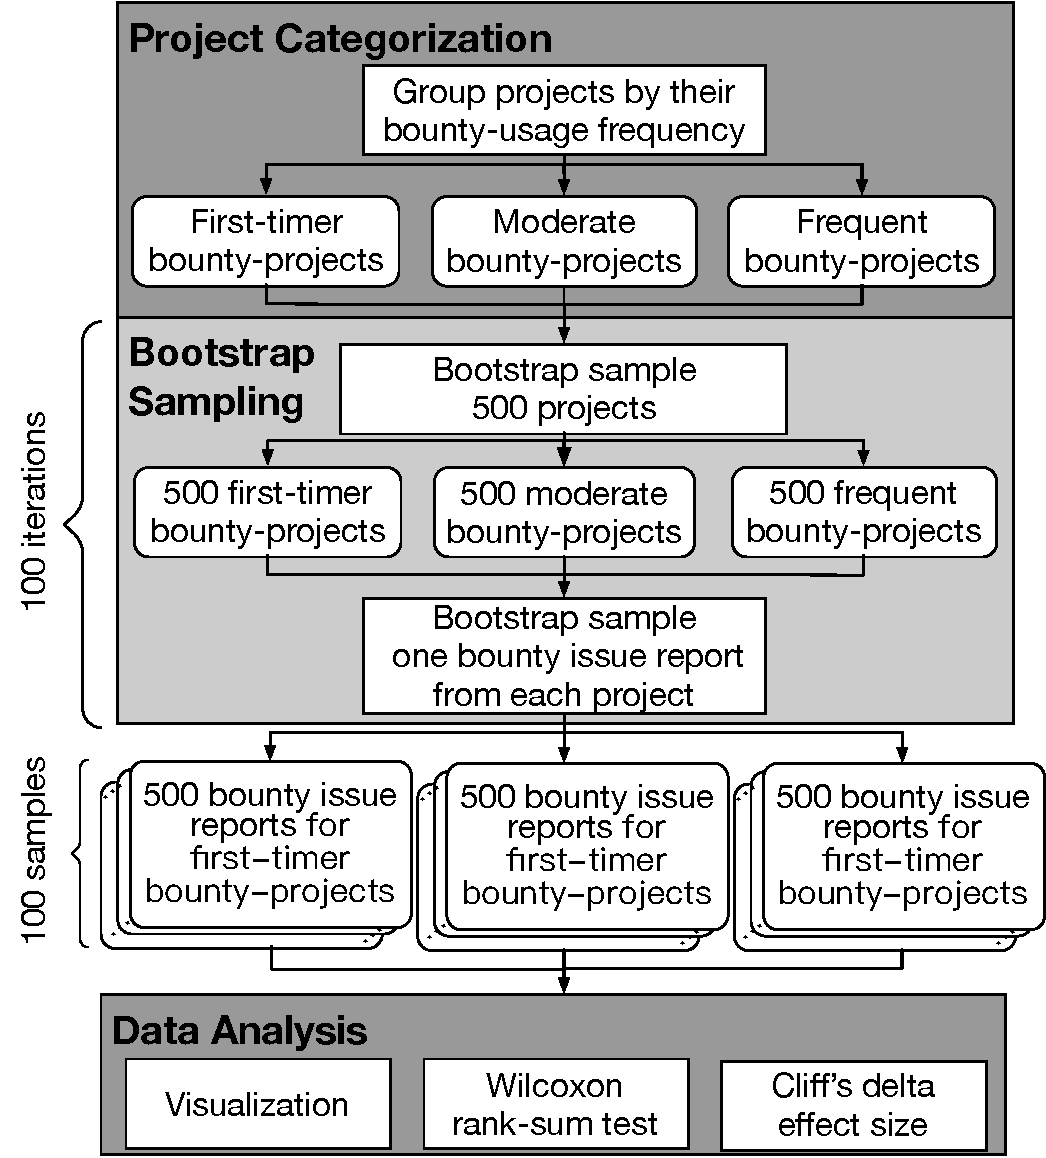
\includegraphics[width=\columnwidth ]{pics/rq1/new/approach}
\caption{An overview of our approach. }
\label{fig:rq1_approach}
\vspace{-0.2in}

\end{figure}

\noindent\textbf{Approach:} Figure~\ref{fig:rq1_approach} gives an overview of our approach. We elaborate on each step below.

\noindent\emph{\textbf{Project categorization:}} Given the variance (see Section~\ref{prestudy}) of the bounty-usage frequency for different projects, it is not advisable to study all the issue reports as one group when we study the bounties at the issue level. Therefore we categorize the projects into the following three groups:

\begin{enumerate}
    \item \textbf{First-timer bounty-projects:} Projects which have only one bounty issue report.
    \item \textbf{Moderate bounty-projects:} Projects which have 2 to 50 bounty issue reports.
    \item \textbf{Frequent bounty-projects:} Projects which have more than 50 bounty issue reports.
\vspace{-0.01in}
\end{enumerate}

It is important to study the bounties in the first-timer bounty-projects, since users of such projects may not have former bounty experience. Insights on the usage (e.g., how large of a bounty should be proposed?) and the impact (e.g., the issue-addressing likelihood) of bounties in these projects may benefit other projects which are new to using bounties. We grouped the projects that have more than 50 bounty issue reports as well since we assume that in such projects the community is more familiar with the use of bounties.
After grouping the projects into the above mentioned three groups we ended up with 768 (65\%) first-timer bounty-projects, 400 (34\%) moderate bounty-projects, and 9 (1\%) frequent bounty-projects. %Note that we study the impact of different thresholds for categorizing moderate bounty-projects and frequent bounty-projects in Section~\ref{sec:threats} and that find our observations still hold.


\noindent\emph{\textbf{Bootstrap sampling:}} After grouping the projects into the three groups, we used a bootstrap sampling approach to sample issue reports across projects. We used bootstrap sampling to reduce the bias that is caused by the unbalanced number of projects across the three groups. We first randomly sampled 500 projects from each group with replacement. Then we randomly sampled one bounty issue report from each sampled project, to avoid a bias towards projects with more issue reports than other projects in the same group. Hence, we sampled 500 bounty issue reports from each of the 3 project groups. To make our results more reliable, we repeated the sampling process 100 times with different random seeds. We ended up with 100 samples with 1,500 issue reports each (500 issue reports for each group).


\noindent\emph{\textbf{Data Analysis:}} For each sample, we calculated the issue-addressing likelihood across the three project groups and plotted the results. To compare the differences between two data distributions (e.g., the differences of the bounty values between successful and failed bounty issue reports), we used the Wilcoxon rank-sum test~\cite{bauer1972constructing}, which does not require the sample to be normally distributed. We consider the two distributions as significantly different when the p-value of the test is smaller than 0.05. Furthermore, we applied Cliff's delta $d$ \cite{long2003ordinal} effect size to quantify the magnitude of the difference. We use the following thresholds for $d$~\cite{romano2006appropriate}: $ \vert d \vert \leq$0.147 (negligible); 0.147 $ < \vert d \vert \leq $0.33 (small); 0.33 $ < \vert d \vert \leq $0.474 (medium); 0.474 $ < \vert d \vert  \leq $1 (large).


\begin{comment}
	
\begin{figure}[t]
\centering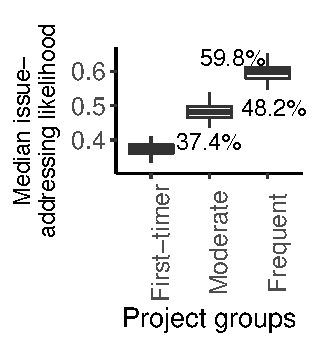
\includegraphics[width=\columnwidth]{pics/rq1/new/rq1_likelihood_ratio500}
\caption{The distribution of the median issue-addressing likelihood for each project group for 100 samples.}
\label{fig:rq1_likelihood_ratio500}
\vspace{-0.1in}
\end{figure}


\begin{figure}[t]
\centering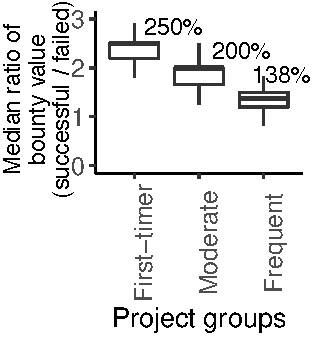
\includegraphics[width=\columnwidth]{pics/rq1/new/rq1_ratio_cp_ou500}
\caption{The distribution of the median ratio of the bounty value of successful bounty issue reports to the value of failed bounty issue reports against three project groups for 100 samples.}
\label{fig:rq1_ratio_cp_ou500}
\vspace{-0.1in}
\end{figure}

\end{comment}

\begin{figure}[t]
    \centering
    \begin{subfigure}[t]{0.45\columnwidth }
        \centering
        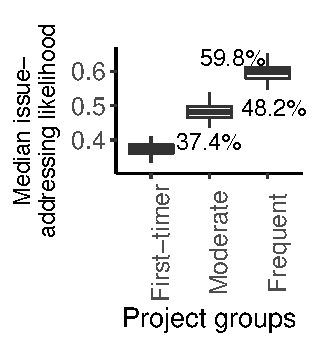
\includegraphics[width=\linewidth]{pics/rq1/new/rq1_likelihood_ratio500}
        \caption{}
		\label{fig:rq1_likelihood_ratio500}
    \end{subfigure}%
    ~
    \begin{subfigure}[t]{0.45\columnwidth}
        \centering
        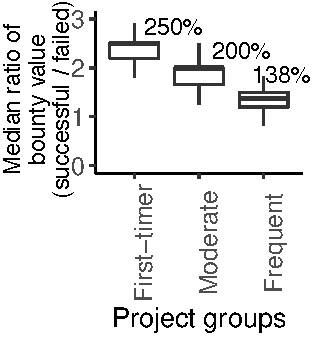
\includegraphics[width=\linewidth]{pics/rq1/new/rq1_ratio_cp_ou500}
        \caption{}
          \label{fig:rq1_ratio_cp_ou500}
    \end{subfigure}
    \vspace{-0.1in}
    \caption{The distribution of the median issue-addressing likelihood (a) and the distribution of the median ratio of the bounty value of successful bounty issue reports to the value of failed bounty issue reports (b) for each project group for 100 samples.
    }
    \vspace{-0.2in}
\end{figure}


\noindent\textbf{Results:}
\textbf{Bounty issue reports in projects which have a higher bounty-usage frequency are more likely to be addressed.} Figure~\ref{fig:rq1_likelihood_ratio500} shows the median issue-addressing likelihood for each project group. We observed a positive relationship between this likelihood and the bounty-usage frequency, which indicates that a bounty issue report is more likely to be addressed in a project with a higher bounty-usage frequency. Our statistical test shows that the issue-addressing likelihood is significantly different across these three groups of projects with a large effect size. One possible explanation is that the lower bounty-usage frequency of a project may indicate that the backers have less experience in proposing a bounty (e.g., at the proper time with a proper value) and the hunters react to bounties less actively than in projects with a higher bounty-usage frequency.



\textbf{The successful bounty issue reports have a relatively higher bounty value than failed bounty issue reports, particularly in the first-timer bounty-projects.}
Figure~\ref{fig:rq1_ratio_cp_ou500} shows that the median ratio (the bounty values of successful reports compared to those of failed reports) is larger than 1 in all 3 project groups. In other words, the successful bounty issue reports have higher bounty values than the failed bounty issue reports. In addition, comparing the ratio across project groups, the first-timer bounty-projects have the largest ratio (2.5) among the three groups, indicating that developers may want more money to address an issue in first-timer bounty-projects than in other projects. Our statistical test results shows that the differences in bounty value between successful and failed bounty issue reports are significant (p-value $<$ 0.05) in the first-timer bounty-projects for all samples with a non-negligible Cliff's delta effect size (72\% samples have a small effect size and 28\% samples have a medium effect size).
In 97\% of the samples of the moderate bounty-projects, the bounty value of successful issue reports is significantly higher than that of failed issues (with a non-negligible effect size in 77\% of the cases).
For the frequent bounty-projects, in 92\% of the samples, the differences were not statistically significant.


\begin{comment}
 \begin{table}[t]
   \centering
   \caption{The comparison of the bounty values between successful bounty issue reports and failed bounty issue reports across three project groups over 100 samples. For example, the differences in bounty value between successful bounty issue reports and failed bounty issue reports in first-timer projects are statistically significant across all the samples (i.e., 100\%). }
     \begin{tabular}{ccccc}
     \toprule
     \multicolumn{1}{c}{} \makecell{\textbf{Bounty-project}\\\textbf{group}}&  \multicolumn{1}{c}{\makecell{\textbf{Wilcoxon}\\\textbf{rank-sum test}}} & \multicolumn{3}{p{3.5cm}}{\textbf{\rule{10pt}{0pt}Cliff's Delta effect size}} \bigstrut\\
    \hline
      & Significant & \multicolumn{1}{p{1.1cm}}{Negligible} & \multicolumn{1}{p{0.1cm}}{Small} & \multicolumn{1}{p{1cm}}{Medium} \bigstrut\\
     \hline
     \textbf{First-timer} &  100\%      & \rule{9pt}{0pt} 0\%     & \rule{3pt}{0pt} 72\%    &\rule{3pt}{0pt}  28\% \\
     \hline
     \textbf{Moderate}&  \rule{4pt}{0pt}97\%        & \rule{9pt}{0pt}23\%    & \rule{5pt}{0pt}76\%    & \rule{9pt}{0pt}1\% \\
     \hline
     \textbf{Frequent} &  \rule{4pt}{0pt}24\%      & \rule{9pt}{0pt}92\%    & \rule{9pt}{0pt}8\%     & \rule{9pt}{0pt}0\% \\
     \hline

     \end{tabular}%
   \label{tab:rq2_value_comparison}%
   \vspace{-0.1in}

 \end{table}%
\end{comment}

One possible explanation is that first-timer bounty-projects may not be as active as moderate and frequent projects. Therefore, backers would be required to propose bounties with higher values to attract enough attention from the community for addressing issues. To investigate this explanation, we examined the activity of the projects in terms of the number of pull requests, issue reports, and commits. Figure~\ref{fig:rq1_activity} shows the distributions of the occurrences of these three activities in each project group.
%The projects in the category with more bounty-usage frequency have more activities.
\textbf{Projects with fewer bounty issue reports are usually less active (in terms of the number of pull requests, issue reports, and commits) than projects with more bounty issue reports.} Another possible explanation is that the backers in the first-timer bounty-projects have no experience in proposing bounties and sometimes overestimate the value of addressing an issue report. In this situation, the overestimated bounty issue reports may attract more attention from the community due to their ``easy money'' and get addressed easier.



\begin{figure}[t]
\centering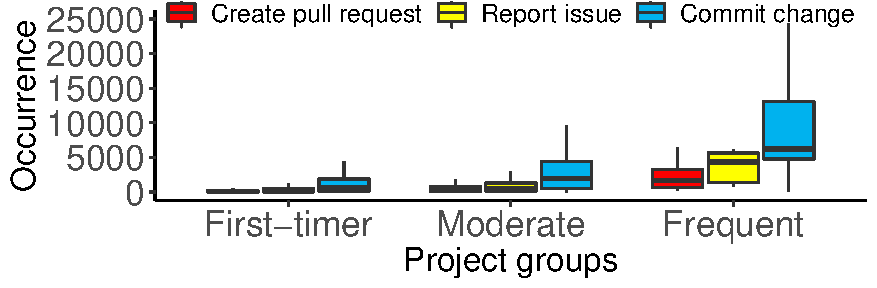
\includegraphics[width=\columnwidth]{pics/rq1/new/rq1_activity}
\caption{The distributions of the occurrences of three activities (i.e., the create pull request, the report issue and the commit change) in each project group.}
\label{fig:rq1_activity}
\vspace{-0.2in}

\end{figure}


\rqbox{The issue-addressing likelihood is higher in projects which used bounties more frequently. Successful bounty issue reports have higher bounty values than failed bounty issue reports in the projects which used bounties less frequently.}
